\documentclass[11pt]{report}

% Paquetes y configuraciones adicionales
\usepackage{graphicx}
\usepackage[export]{adjustbox}
\usepackage{caption}
\usepackage{float}
\usepackage{titlesec}
\usepackage{geometry}
\usepackage[hidelinks]{hyperref}
\usepackage{titling}
\usepackage{titlesec}
\usepackage{parskip}
\usepackage{wasysym}
\usepackage{tikzsymbols}
\usepackage{fancyvrb}
\usepackage{xurl}
\usepackage{hyperref}
\usepackage{subcaption}

\usepackage{listings}
\usepackage{xcolor}

\usepackage[spanish]{babel}

\newcommand{\subtitle}[1]{
  \posttitle{
    \par\end{center}
    \begin{center}\large#1\end{center}
    \vskip0.5em}
}

% Configura los márgenes
\geometry{
  left=2cm,   % Ajusta este valor al margen izquierdo deseado
  right=2cm,  % Ajusta este valor al margen derecho deseado
  top=3cm,
  bottom=3cm,
}

% Configuración de los títulos de las secciones
\titlespacing{\section}{0pt}{\parskip}{\parskip}
\titlespacing{\subsection}{0pt}{\parskip}{\parskip}
\titlespacing{\subsubsection}{0pt}{\parskip}{\parskip}

% Redefinir el formato de los capítulos y añadir un punto después del número
\makeatletter
\renewcommand{\@makechapterhead}[1]{%
  \vspace*{0\p@} % Ajusta este valor para el espaciado deseado antes del título del capítulo
  {\parindent \z@ \raggedright \normalfont
    \ifnum \c@secnumdepth >\m@ne
        \huge\bfseries \thechapter.\ % Añade un punto después del número
    \fi
    \interlinepenalty\@M
    #1\par\nobreak
    \vspace{10pt} % Ajusta este valor para el espacio deseado después del título del capítulo
  }}
\makeatother

% Configura para que cada \chapter no comience en una pagina nueva
\makeatletter
\renewcommand\chapter{\@startsection{chapter}{0}{\z@}%
    {-3.5ex \@plus -1ex \@minus -.2ex}%
    {2.3ex \@plus.2ex}%
    {\normalfont\Large\bfseries}}
\makeatother

% Configurar los colores para el código
\definecolor{codegreen}{rgb}{0,0.6,0}
\definecolor{codegray}{rgb}{0.5,0.5,0.5}
\definecolor{codepurple}{rgb}{0.58,0,0.82}
\definecolor{backcolour}{rgb}{0.95,0.95,0.92}

% Configurar el estilo para el código
\lstdefinestyle{mystyle}{
  backgroundcolor=\color{backcolour},   
  commentstyle=\color{codegreen},
  keywordstyle=\color{magenta},
  numberstyle=\tiny\color{codegray},
  stringstyle=\color{codepurple},
  basicstyle=\ttfamily\footnotesize,
  breakatwhitespace=false,         
  breaklines=true,                 
  captionpos=b,                    
  keepspaces=true,                 
  numbers=left,                    
  numbersep=5pt,                  
  showspaces=false,                
  showstringspaces=false,
  showtabs=false,                  
  tabsize=2
}

%==============================================================================
% Cosas para la documentación LateX
% % Sangría
% \setlength{\parindent}{1em}Texto

% % Quitar sangría
% \noindent

% % Punto
% \CIRCLE \ \ \textbf{Texto} \emph{algo}
% \begin{itemize}
%   \item \textbf{Negrita:} Texto
%   \item \textbf{Negrita:} Texto
% \end{itemize}

% % Introducir código
% \begin{center}
%   \begin{BVerbatim}
%     ... Código
%   \end{BVerbatim}
% \end{center}

% Poner una imagen
% \begin{figure}[H]
%   \centering
%   \includegraphics[scale=0.55]{img/}
%   \caption{Exportación de la base de datos en formato sql}
%   \label{fig:exportación de la base de datos en formato sql}
% \end{figure}

% Poner dos imágenes
% \begin{figure}[H]
%   \begin{subfigure}{0.5\textwidth}
%     \centering
%     \includegraphics[scale=0.45]{img/}
%     \caption{Texto imagen 1}
%   \end{subfigure}%
%   \begin{subfigure}{0.5\textwidth}
%     \centering
%     \includegraphics[scale=0.45]{img/}
%     \caption{Texto imagen 2}
%   \end{subfigure}
%   \caption{Texto general}
% \end{figure}

% % Poner una tabla
% \begin{table}[H]
%   \centering
%   \begin{tabular}{|c|c|c|c|}
%     \hline
%     \textbf{Campo 1} & \textbf{Campo 2} & \textbf{Campo 3} & \textbf{Campo 4} \\ \hline
%     Texto & Texto & Texto & Texto \\ \hline
%     Texto & Texto & Texto & Texto \\ \hline
%     Texto & Texto & Texto & Texto \\ \hline
%     Texto & Texto & Texto & Texto \\ \hline
%   \end{tabular}
%   \caption{Nombre de la tabla}
%   \label{tab:nombre de la tabla}
% \end{table}

% % Poner codigo de un lenguaje a partir de un archivo
% \lstset{style=mystyle}
% The next code will be directly imported from a file
% \lstinputlisting[language=Python]{code.py}

% “Texto entre comillas dobles”

%==============================================================================

\begin{document}

% Portada del informe
\title{Diseño y simulación de máquinas de Turing en JFLAP}
\subtitle{Computabilidad y Algoritmia}
\author{Cheuk Kelly Ng Pante (alu0101364544@ull.edu.es)}
\date{12/11/2024}

\maketitle

\pagestyle{empty} % Desactiva la numeración de página para el índice

% Índice
\tableofcontents

% Nueva página
\cleardoublepage

\pagestyle{plain} % Vuelve a activar la numeración de página
\setcounter{page}{1} % Reinicia el contador de página a 1

% Secciones del informe
% Capitulo 1
\chapter{Ejercicios de diseño de máquinas de Turing}
% Ejercicio 1
\section{Diseñar y simular en JFLAP máquinas de Turing que acepten el lenguaje $L = \{a^nb^nc^n \mid n \geq 0\}.$}
\subsection{Diseño de una cinta}
\begin{itemize}
  \item \textbf{Descripción y diseño:} Esta máquina de Turing tiene una cinta, lo que hace es ir marcando las $a$ con
        una $X$, las $b$ con una $Y$ y las $c$ con una $Z$. Luego, regresa al inicio de
        la cadena y repite el proceso hasta que no haya más $a$'s, $b$'s y $c$'s.
        Cuando termina de procesar la cadena, la máquina verifica que no haya
        caracteres restantes sin marcar. El diseño de la máquina de Turing es el siguiente:

        \begin{figure}[H]
          \centering
          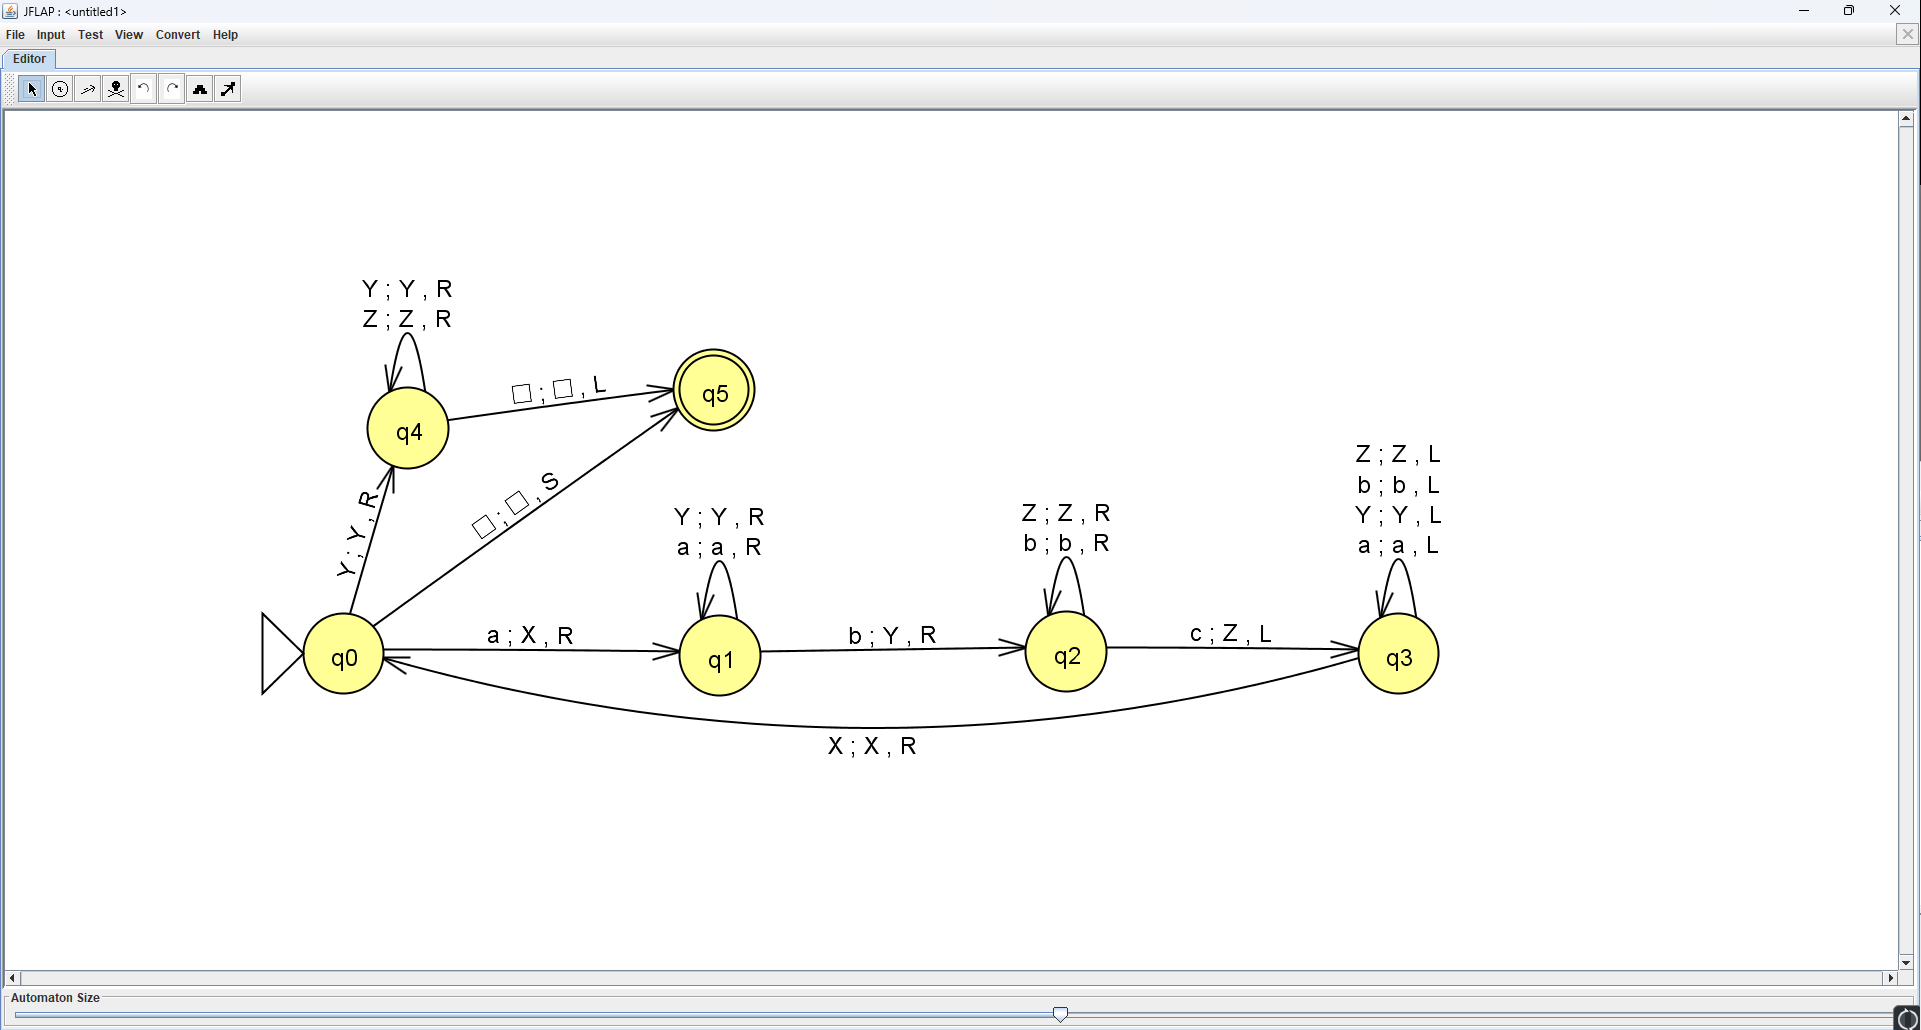
\includegraphics[scale=0.33]{img/MT_01_one_ribbon.png}
          \caption{Máquina de Turing que acepta el lenguaje $L = \{a^nb^nc^n \mid n \geq 0\}$ de una cinta.}
          \label{fig:maquina de turing que acepta el lenguaje L = {a^nb^nc^n | n >= 0}}
        \end{figure}

  \newpage

  \item \textbf{Simulación:} La simulación de la máquina de Turing con algunas cadenas:
        \begin{figure}[H]
          \centering
          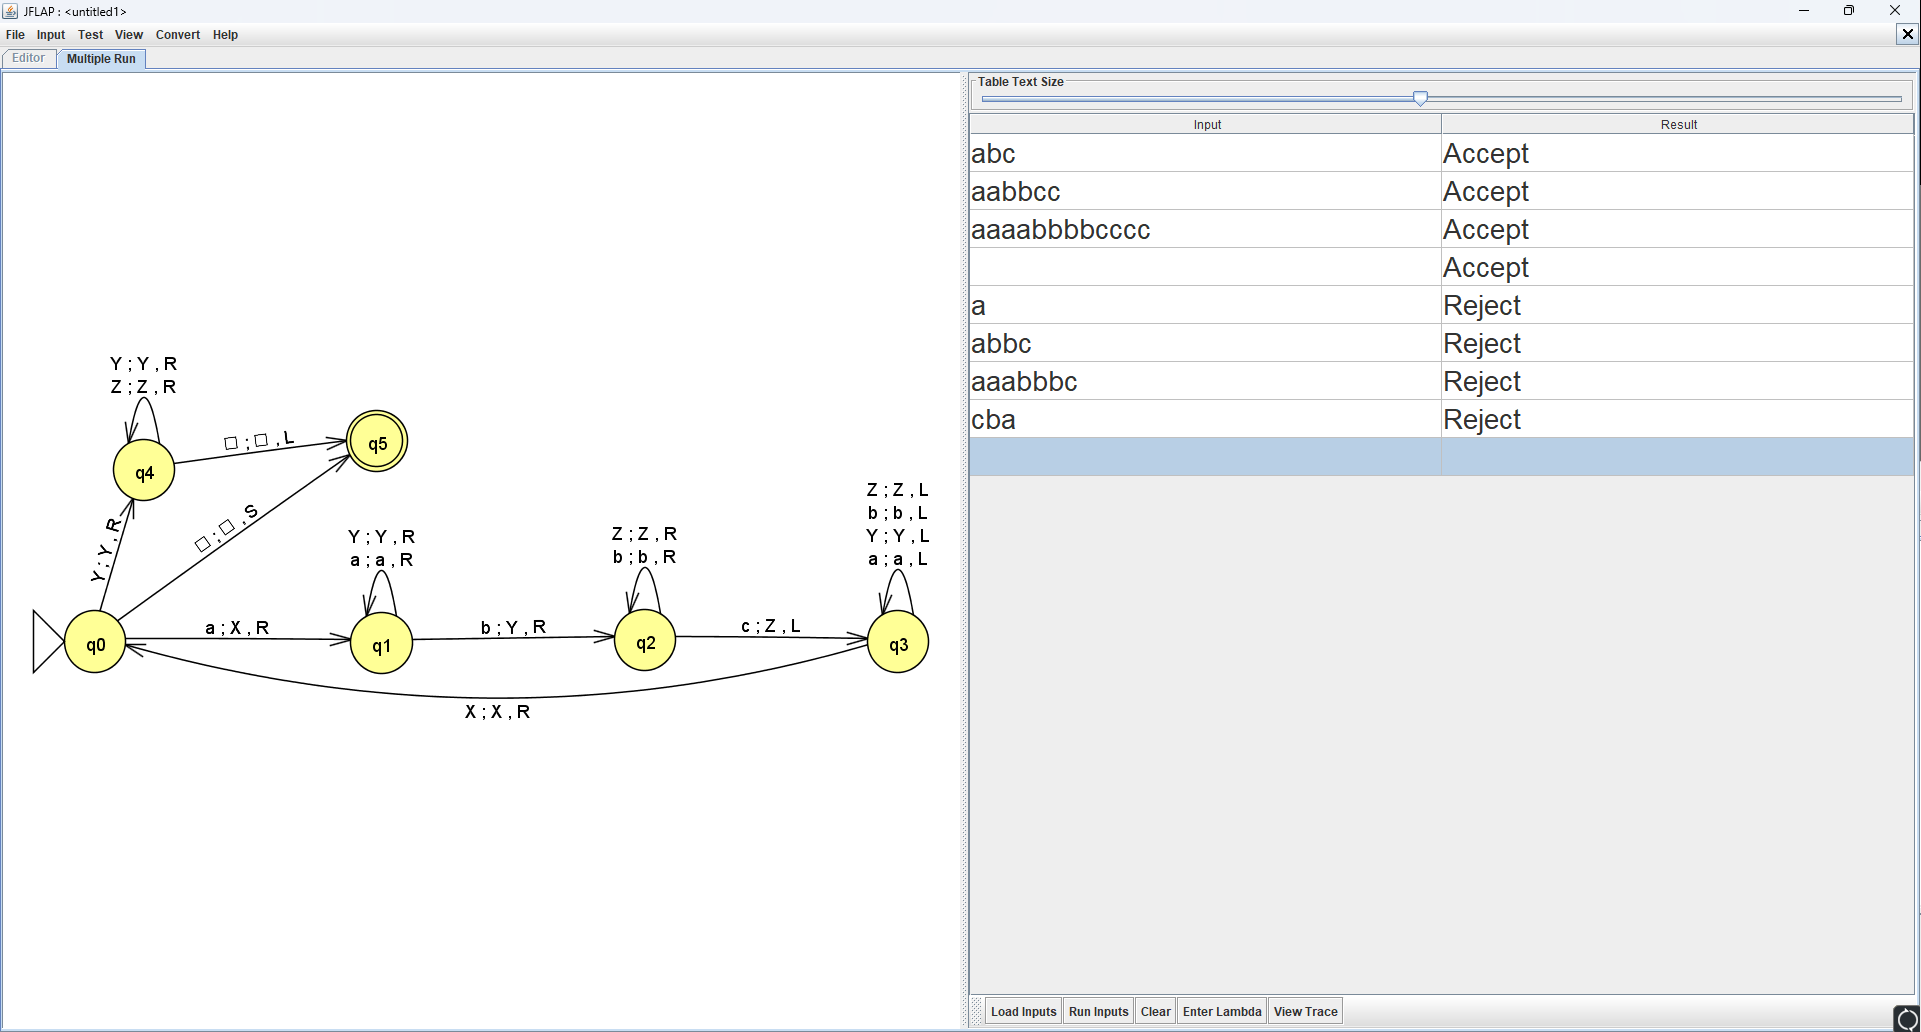
\includegraphics[scale=0.33]{img/MT_01_one_ribbon_simulation.png}
          \caption{Simulación de la máquina de Turing que acepta el lenguaje $L = \{a^nb^nc^n \mid n \geq 0\}$ de una cinta.}
          \label{fig:simulacion de la maquina de turing que acepta el lenguaje L = {a^nb^nc^n | n >= 0}}
        \end{figure}
\end{itemize}

\newpage

\subsection{Diseño de multiples cintas}
\begin{itemize}
  \item \textbf{Descripción y diseño:} Esta máquina de Turing tiene dos cintas, la primera se encarga de procesar la cadena y la segunda en hacer hacer una copia de tantos $a$'s que hay y luego así contar si hay el mismo número de $b$'s y $c$'s. El diseño de la máquina de Turing es el siguiente:

        \begin{figure}[H]
          \centering
          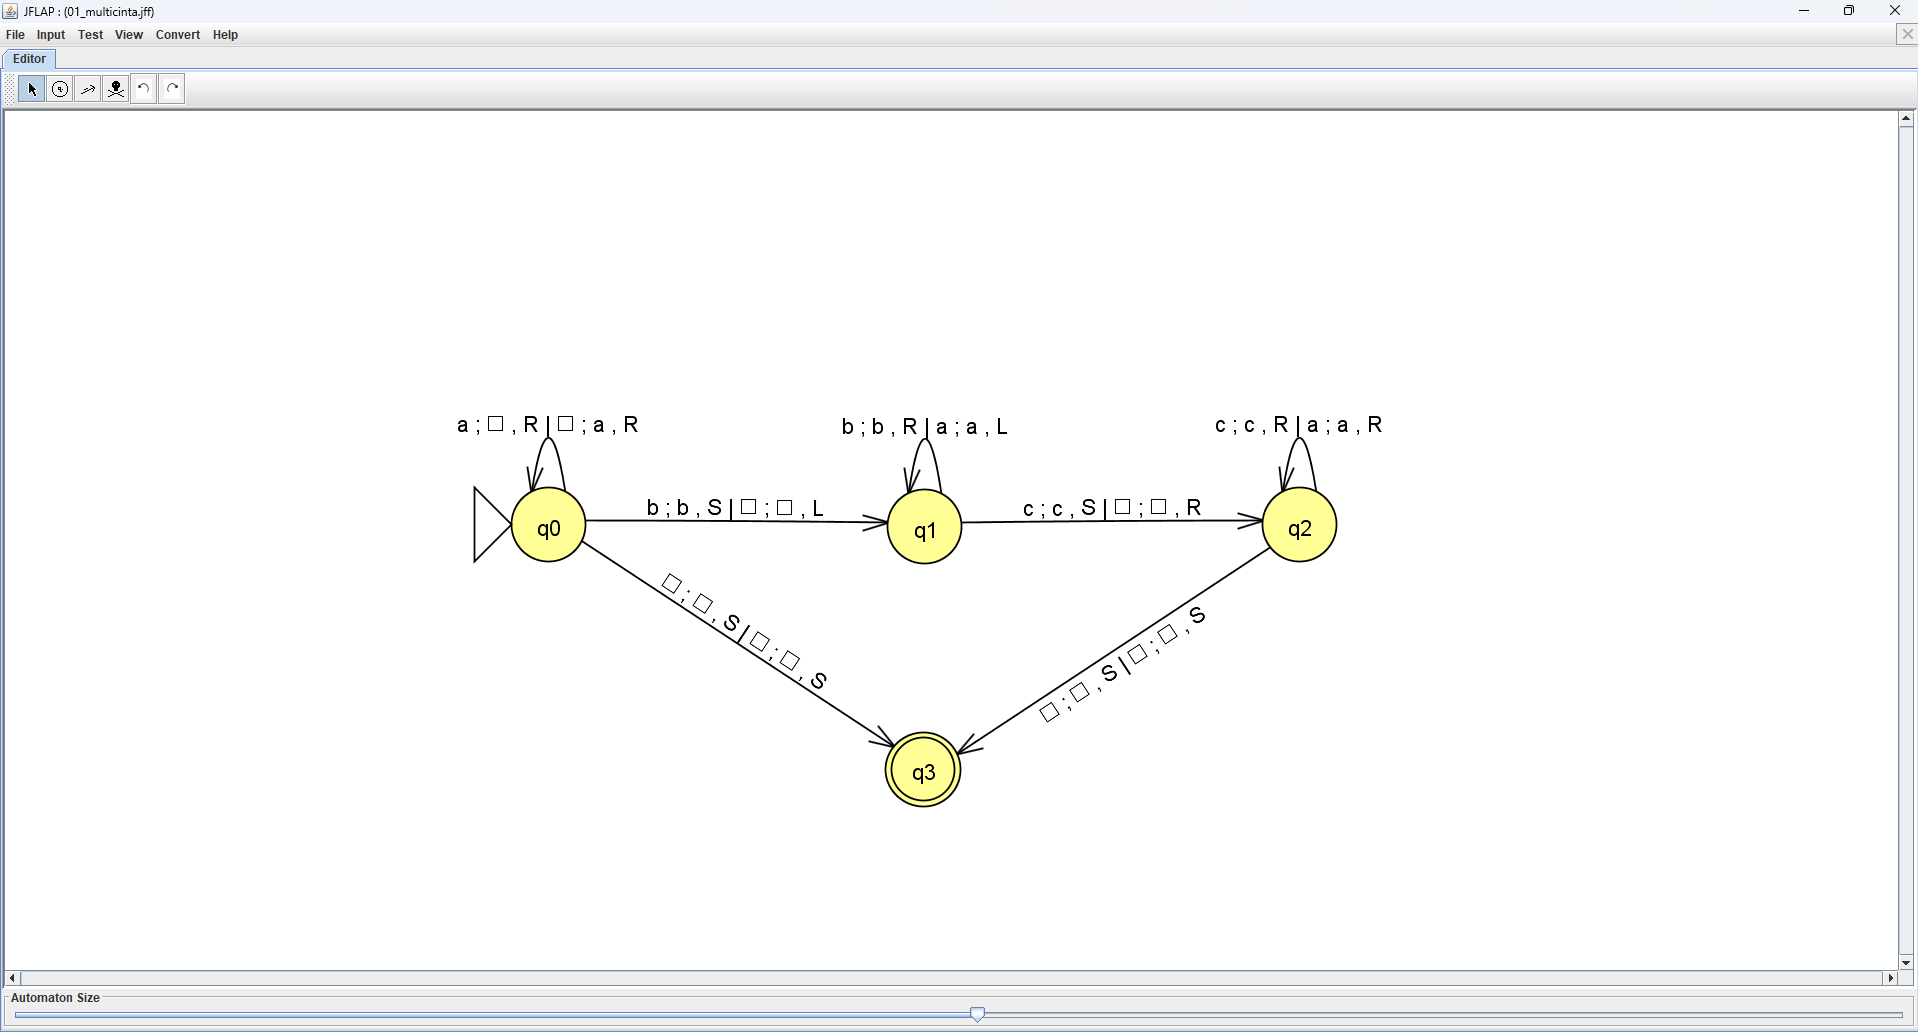
\includegraphics[scale=0.33]{img/MT_01_multiple_ribbon.png}
          \caption{Máquina de Turing que acepta el lenguaje $L = \{a^nb^nc^n \mid n \geq 0\}$ de dos cintas.}
          \label{fig:maquina de turing que acepta el lenguaje L = {a^nb^nc^n | n >= 0}}
        \end{figure}

  \newpage

  \item \textbf{Simulación:} La simulación de la máquina de Turing con algunas cadenas:
        \begin{figure}[H]
          \centering
          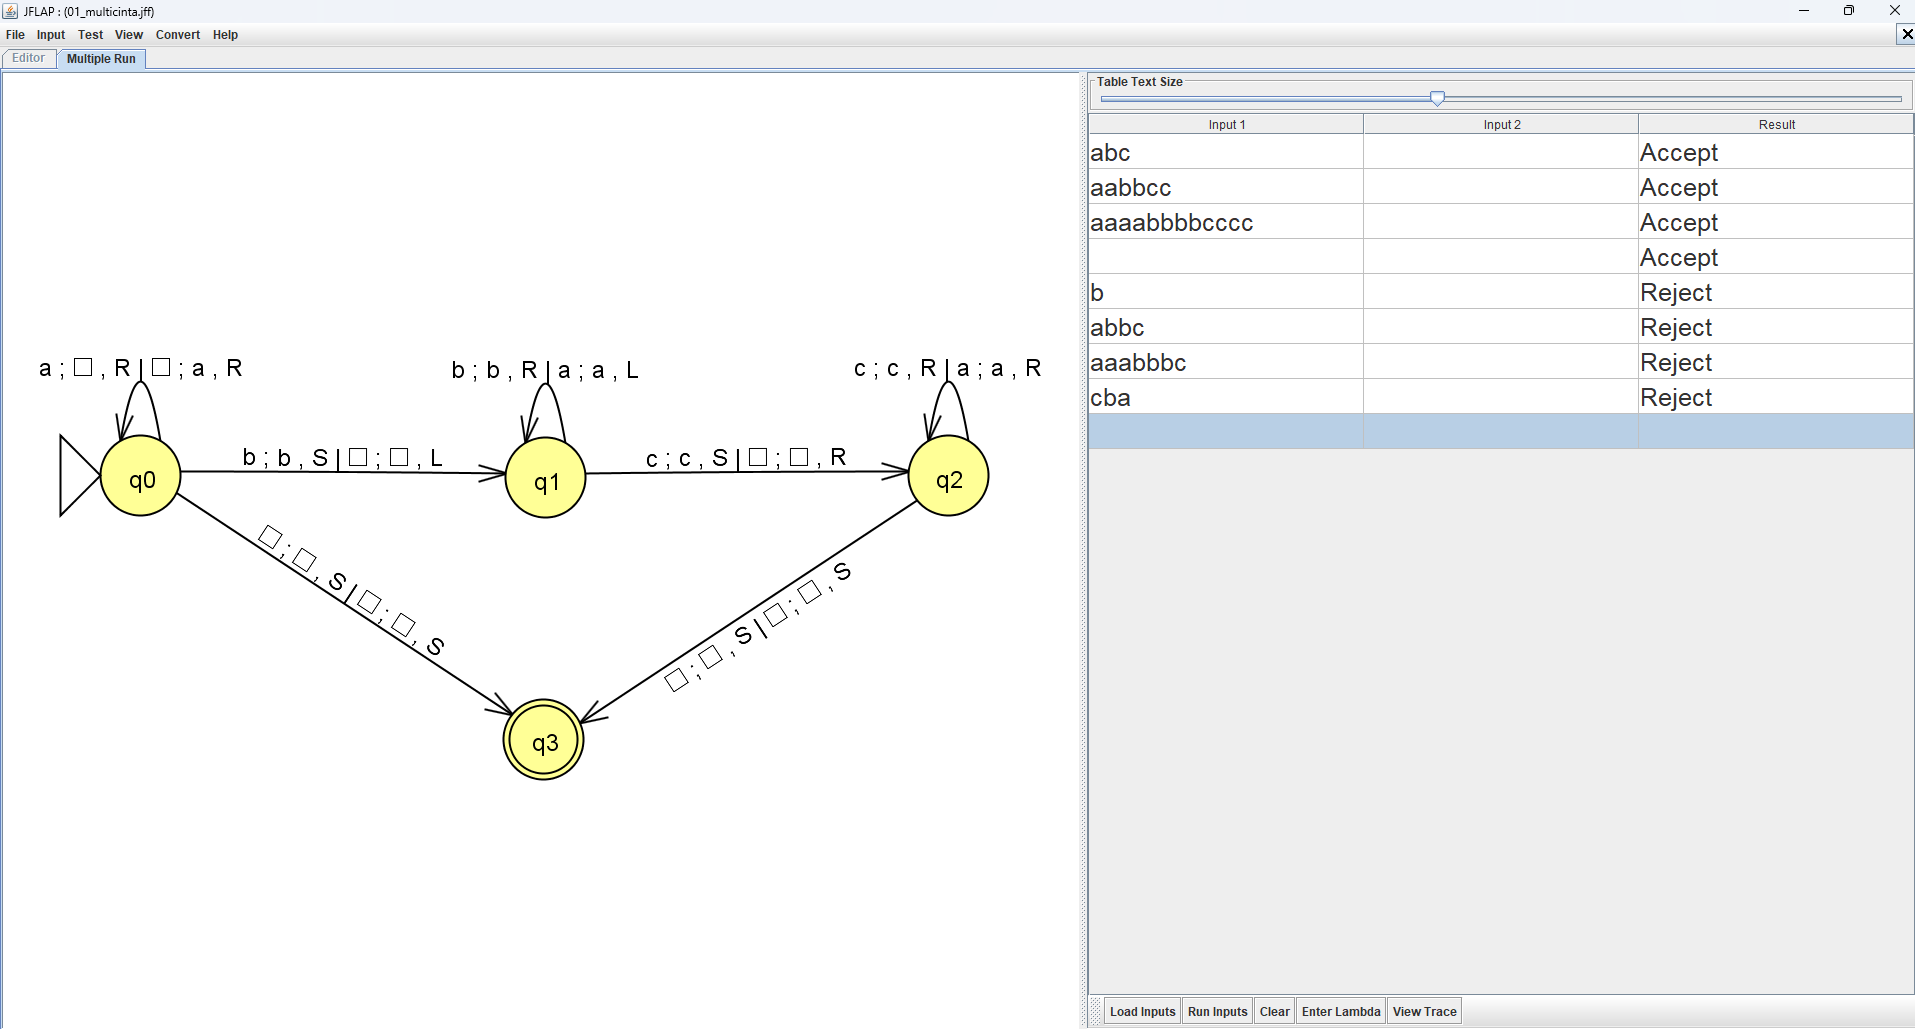
\includegraphics[scale=0.33]{img/MT_01_multiple_ribbon_simulation.png}
          \caption{Simulación de la máquina de Turing que acepta el lenguaje $L = \{a^nb^nc^n \mid n \geq 0\}$ de dos cintas.}
          \label{fig:simulacion de la maquina de turing que acepta el lenguaje L = {a^nb^nc^n | n >= 0}}
        \end{figure}
\end{itemize}

\newpage

% Ejercicio 2
\section{Diseñar y simular en JFLAP máquinas de Turing que acepten el lenguaje $L = \{a^nb^mc^{n+m} \mid n \geq 0, m \geq 0\}$}
\subsection{Diseño de una cinta}
\begin{itemize}
  \item \textbf{Descripción y diseño:} Esta máquina de Turing tiene una cinta, lo que hace es ir marcando por cada $a$ una $c$ y por cada $b$ una $c$. Luego, regresa al inicio de la cadena y repite el proceso hasta que no haya más $a$'s y $b$'s. Cuando termina de procesar la cadena, la máquina verifica que no haya caracteres restantes sin marcar. El diseño de la máquina de Turing es el siguiente:

        \begin{figure}[H]
          \centering
          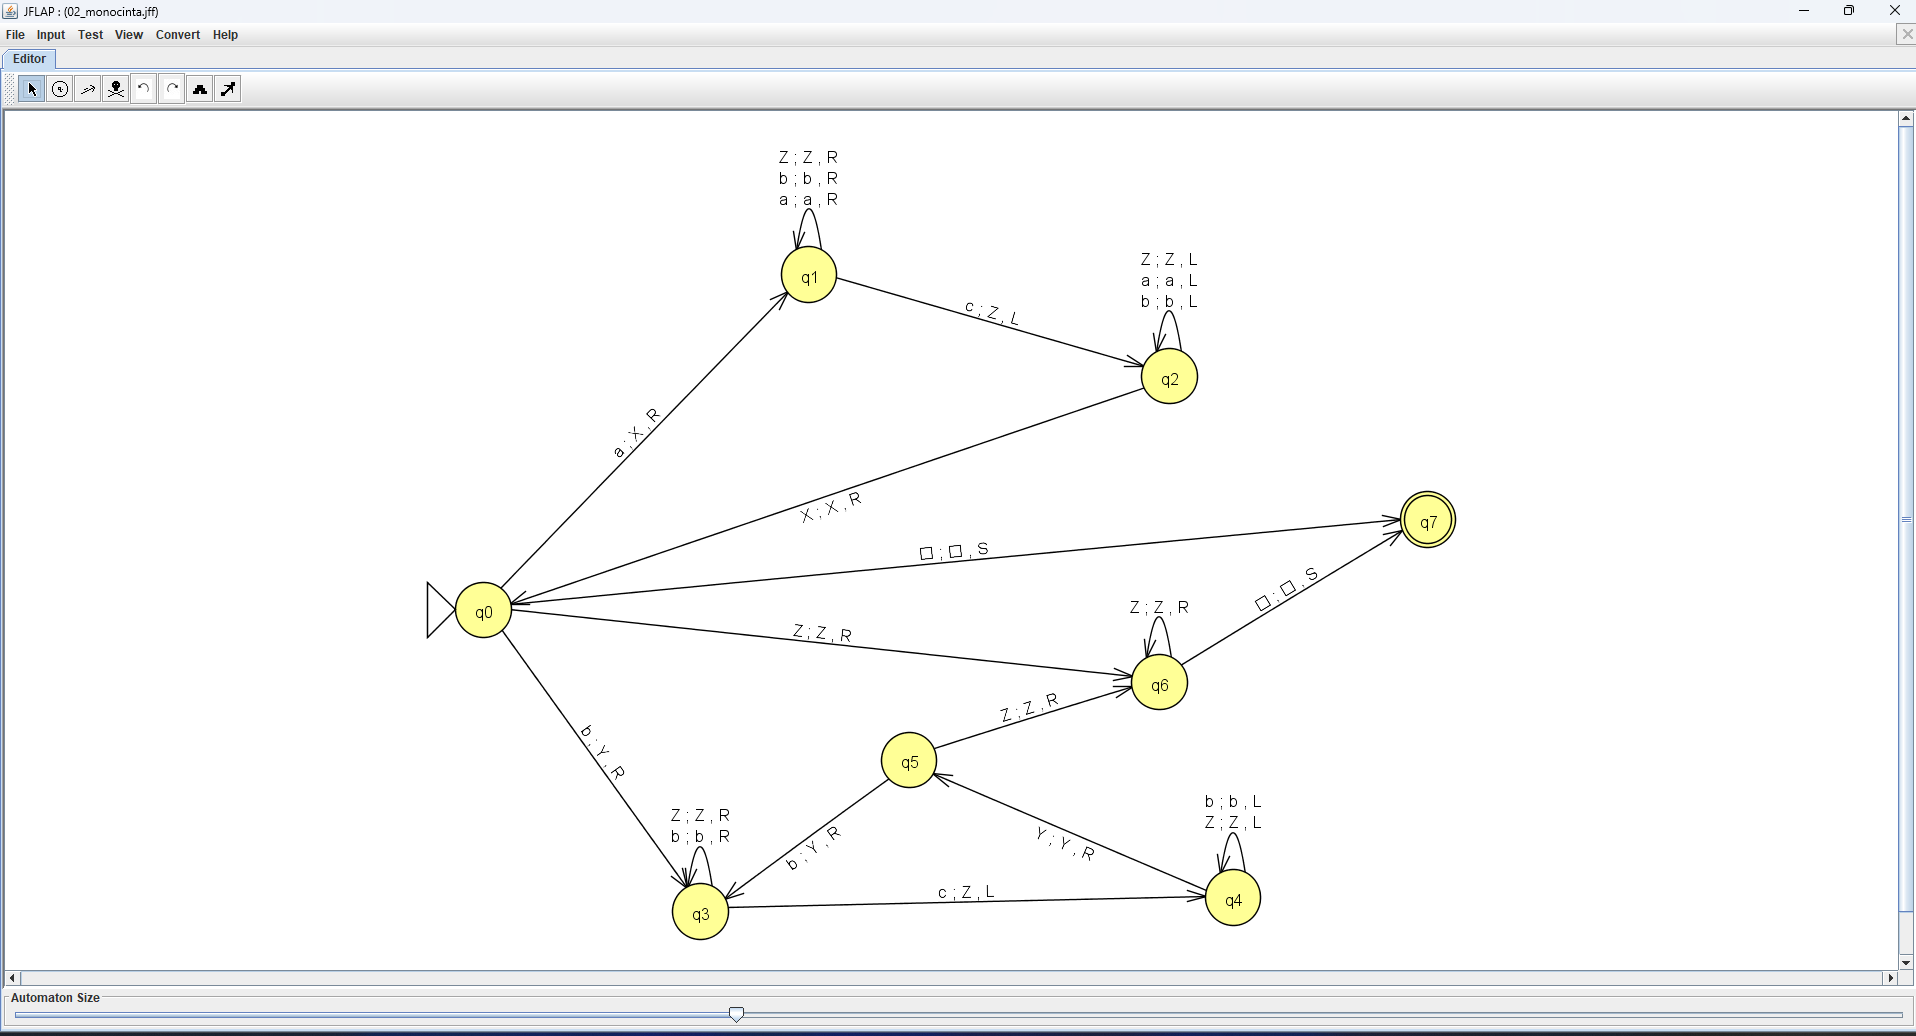
\includegraphics[scale=0.33]{img/MT_02_one_ribbon.png}
          \caption{Máquina de Turing que acepta el lenguaje $L = \{a^nb^mc^{n+m} \mid n \geq 0, m \geq 0\}$ de una cinta.}
          \label{fig:maquina de turing que acepta el lenguaje L = {a^nb^mc^{n+m} | n >= 0, m >= 0}}
        \end{figure}

  \newpage

  \item \textbf{Simulación:} La simulación de la máquina de Turing con algunas cadenas:
        \begin{figure}[H]
          \centering
          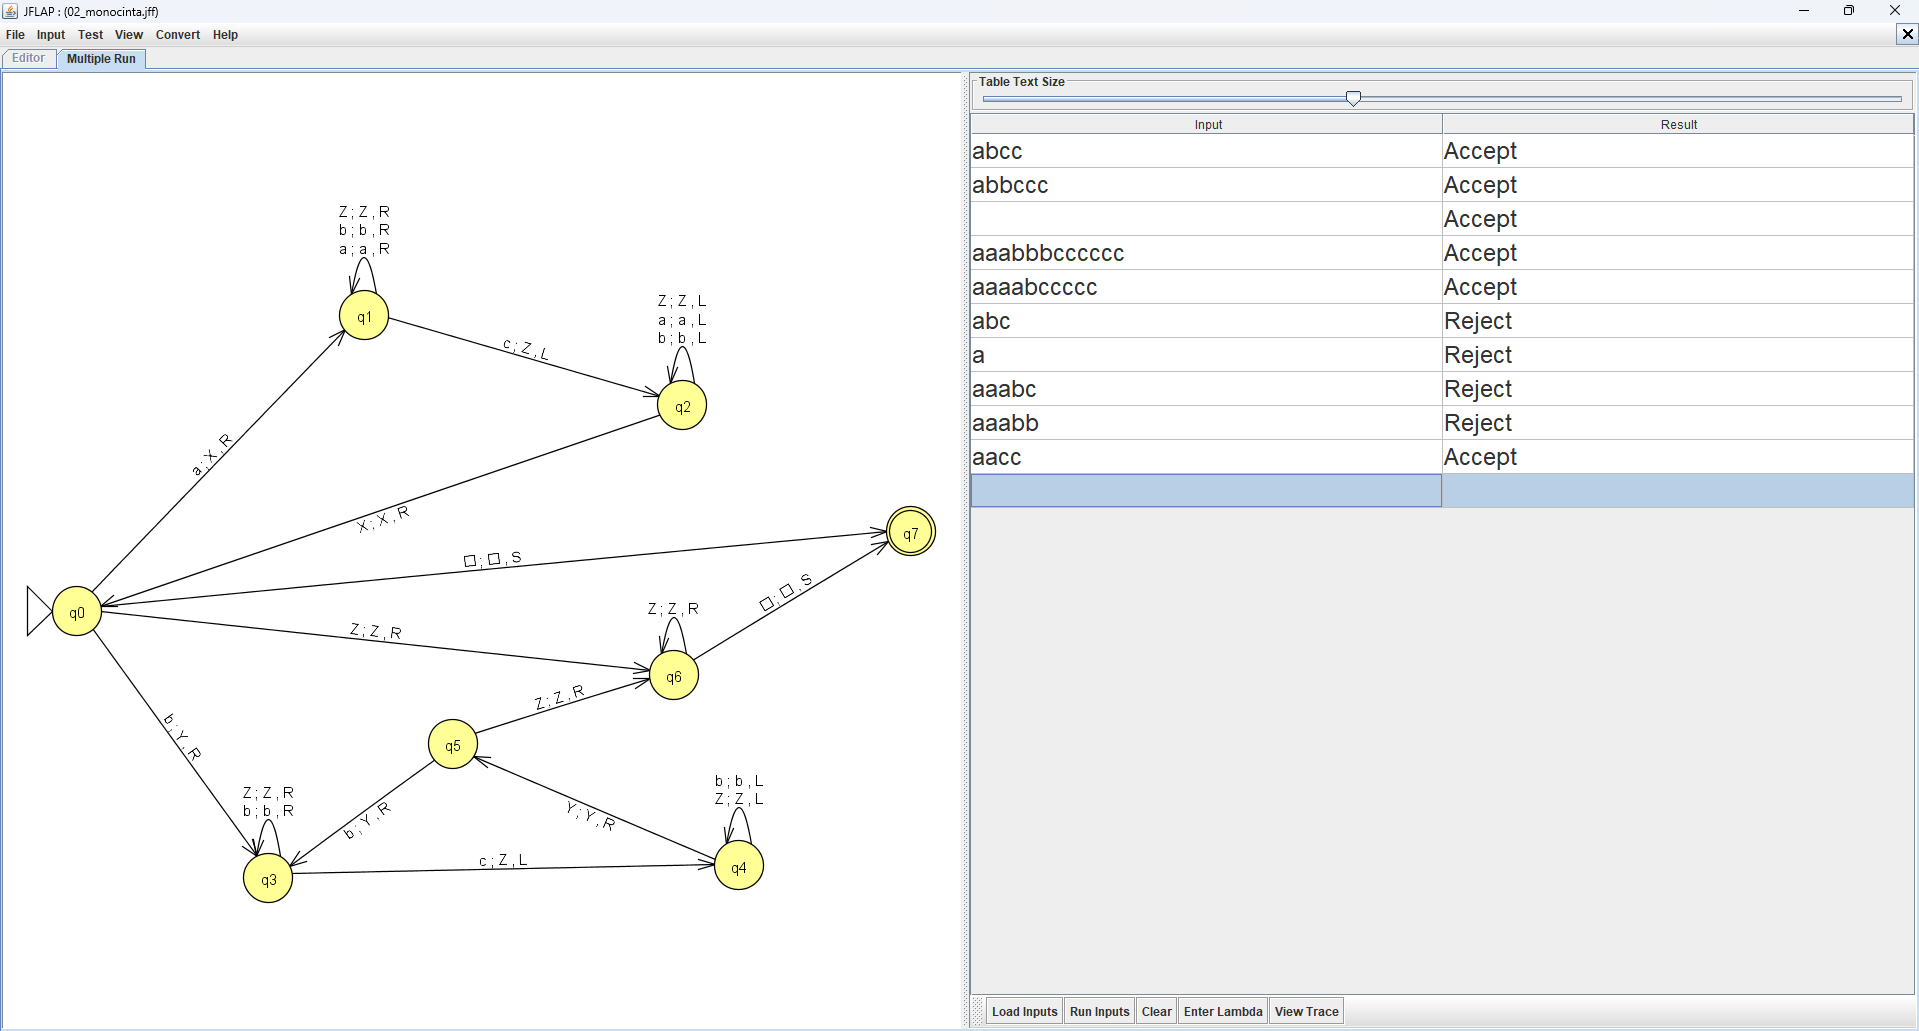
\includegraphics[scale=0.33]{img/MT_02_one_ribbon_simulation.png}
          \caption{Simulación de la máquina de Turing que acepta el lenguaje $L = \{a^nb^mc^{n+m} \mid n \geq 0, m \geq 0\}$ de una cinta.}
          \label{fig:simulacion de la maquina de turing que acepta el lenguaje L = {a^nb^mc^{n+m} | n >= 0, m >= 0}}
        \end{figure}
\end{itemize}

\newpage

\subsection{Diseño de multiples cintas}
\begin{itemize}
  \item \textbf{Descripción y diseño:} Esta máquina de Turing tiene dos cintas, la primera se encarga de procesar la cadena y la segunda en hacer una copia de tantos $a$'s que hay y luego así contar si hay el mismo número de $b$'s y $c$'s. El diseño de la máquina de Turing es el siguiente:

        \begin{figure}[H]
          \centering
          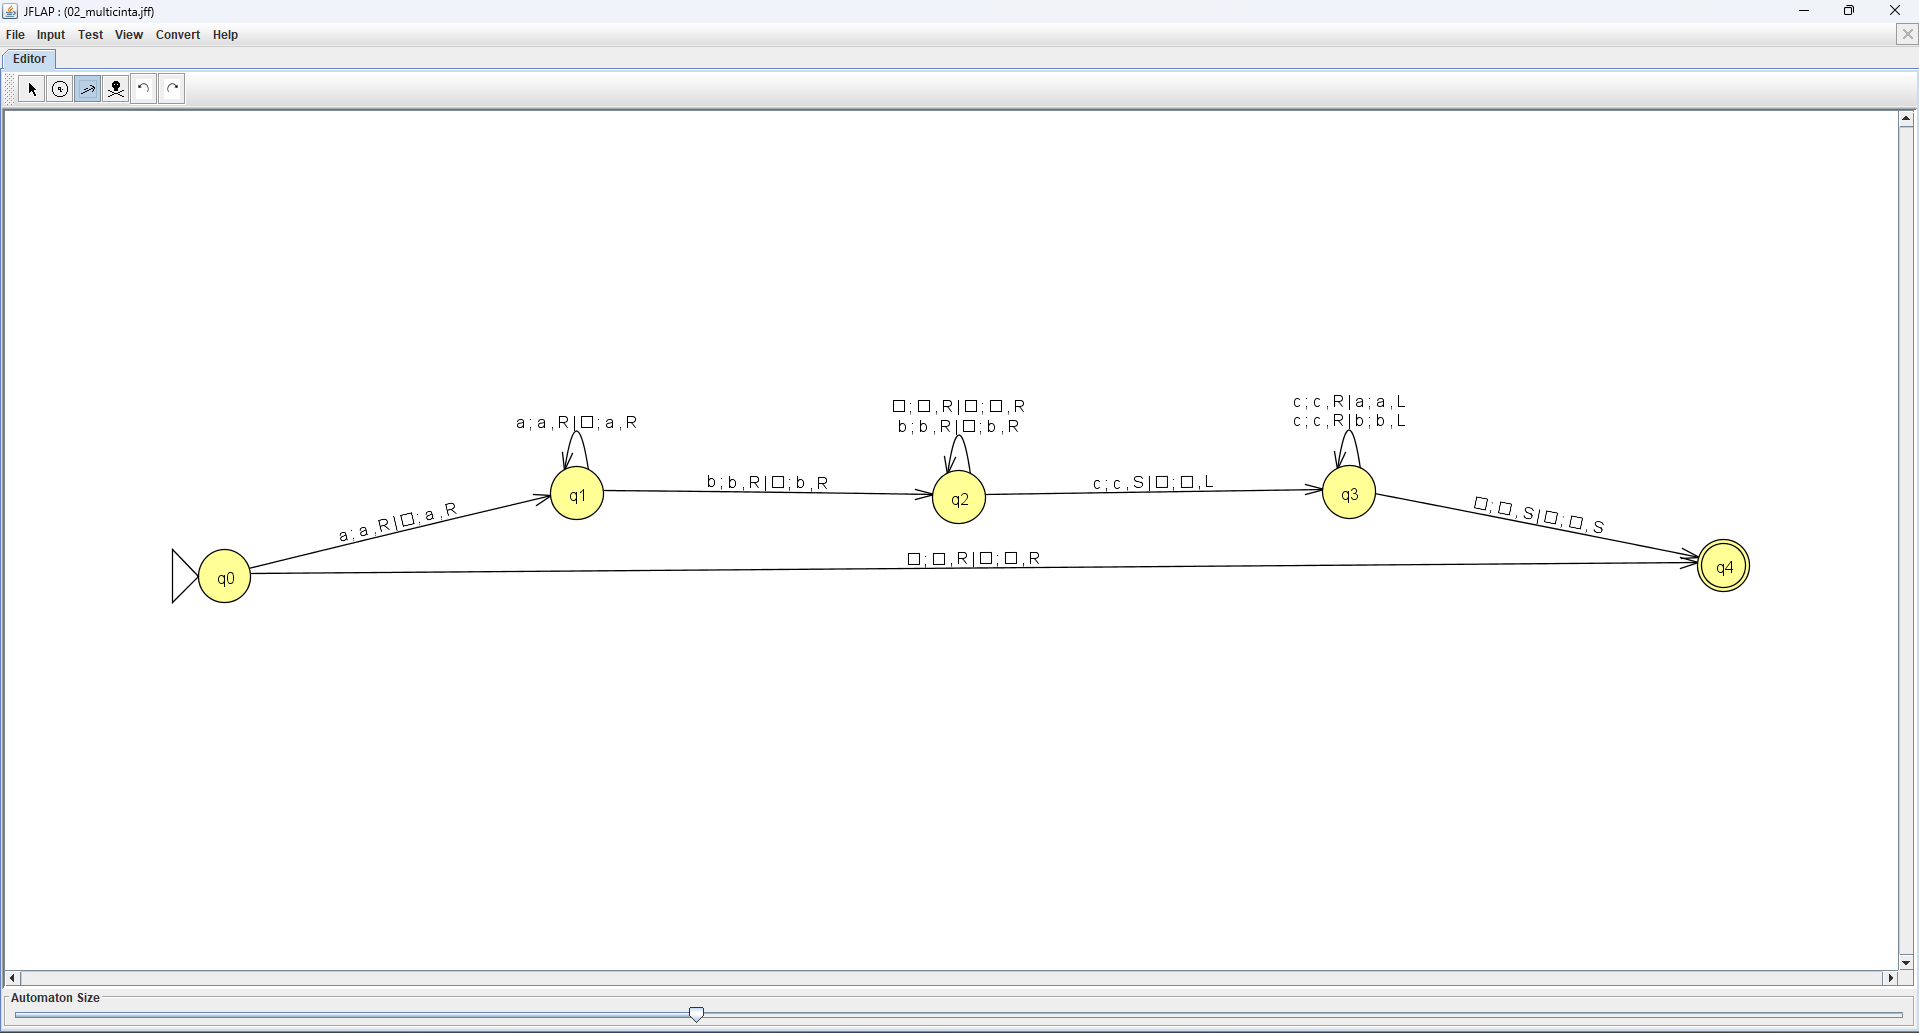
\includegraphics[scale=0.3]{img/MT_02_multiple_ribbon.png}
          \caption{Máquina de Turing que acepta el lenguaje $L = \{a^nb^mc^{n+m} \mid n \geq 0, m \geq 0\}$ de dos cintas.}
          \label{fig:maquina de turing que acepta el lenguaje L = {a^nb^mc^{n+m} | n >= 0, m >= 0}}
        \end{figure}

  \newpage

  \item \textbf{Simulación:} La simulación de la máquina de Turing con algunas cadenas:
        \begin{figure}[H]
          \centering
          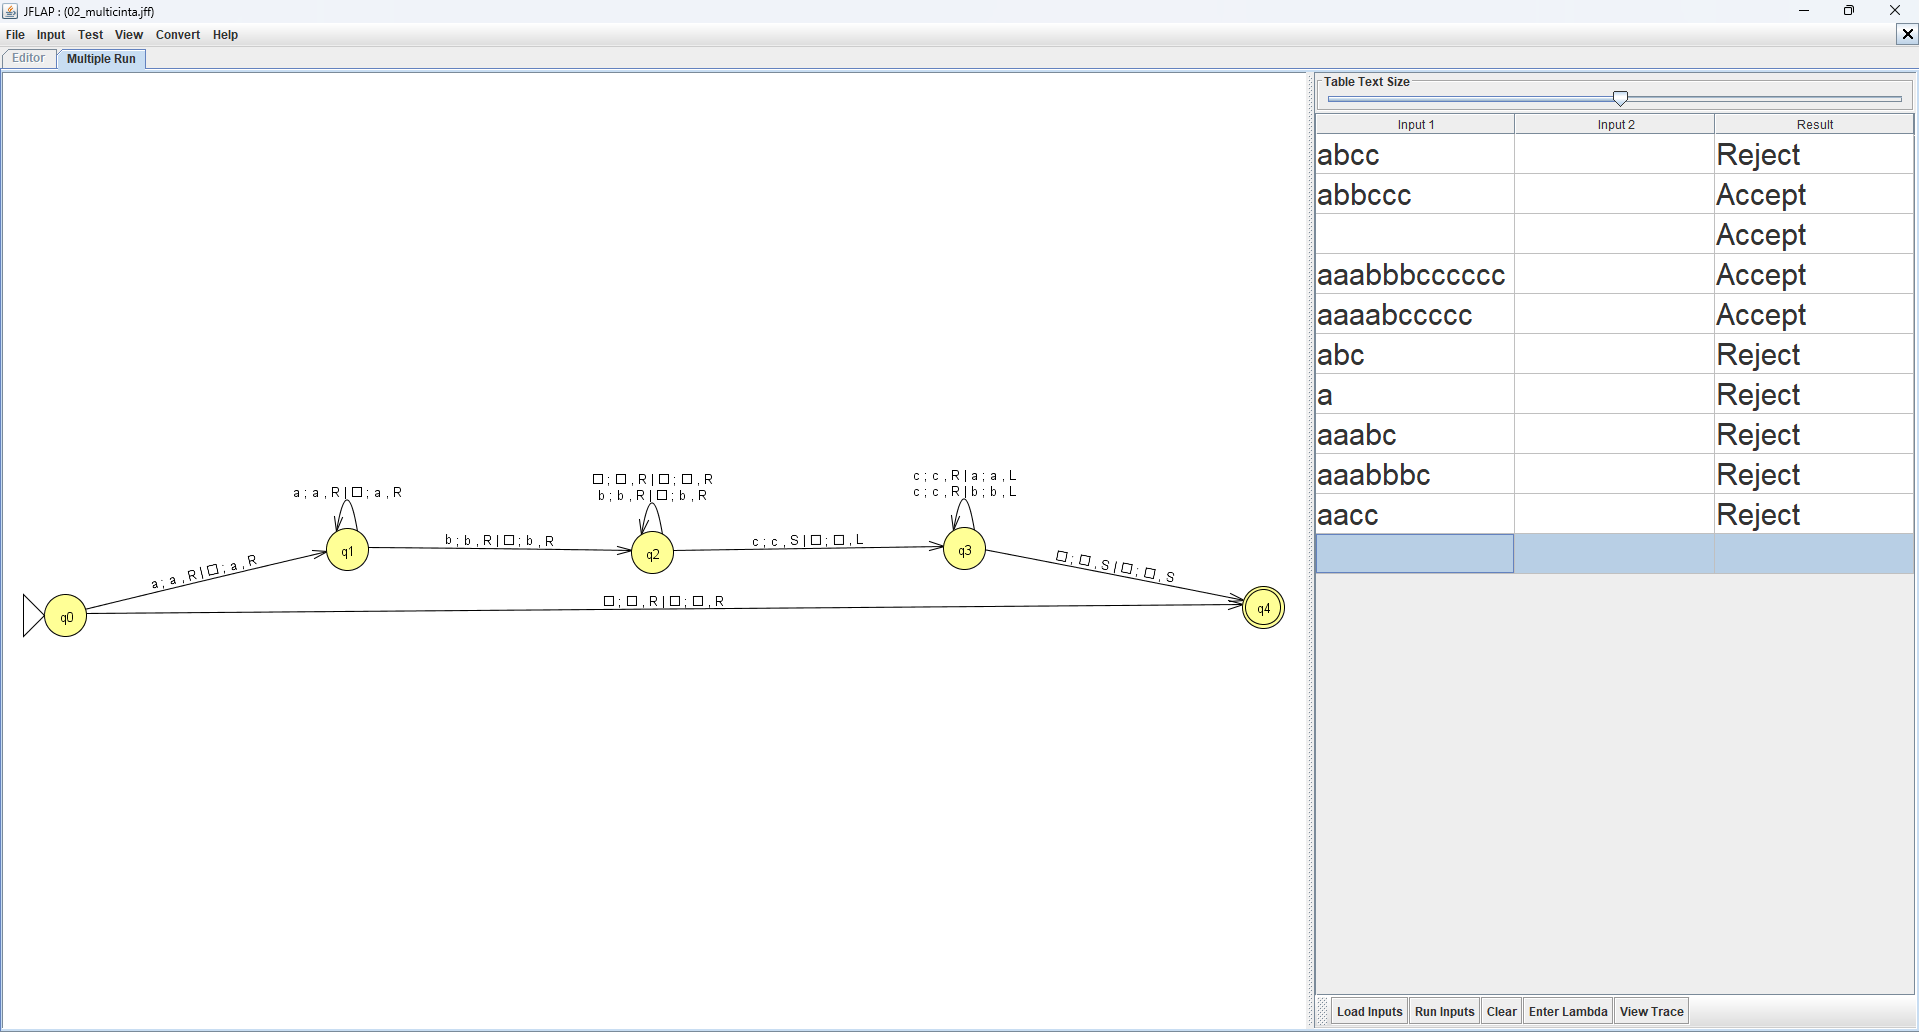
\includegraphics[scale=0.3]{img/MT_02_multiple_ribbon_simulation.png}
          \caption{Simulación de la máquina de Turing que acepta el lenguaje $L = \{a^nb^mc^{n+m} \mid n \geq 0, m \geq 0\}$ de dos cintas.}
          \label{fig:simulacion de la maquina de turing que acepta el lenguaje L = {a^nb^mc^{n+m} | n >= 0, m >= 0}}
        \end{figure}

        Al ejecutar la máquina de Turing con la cadena $abcc$ en la simulacion múltiple rechaza la cadena, pero si la ejecutamos con la cadena de forma individual, la acepta. 
        \begin{figure}[H]
          \centering
          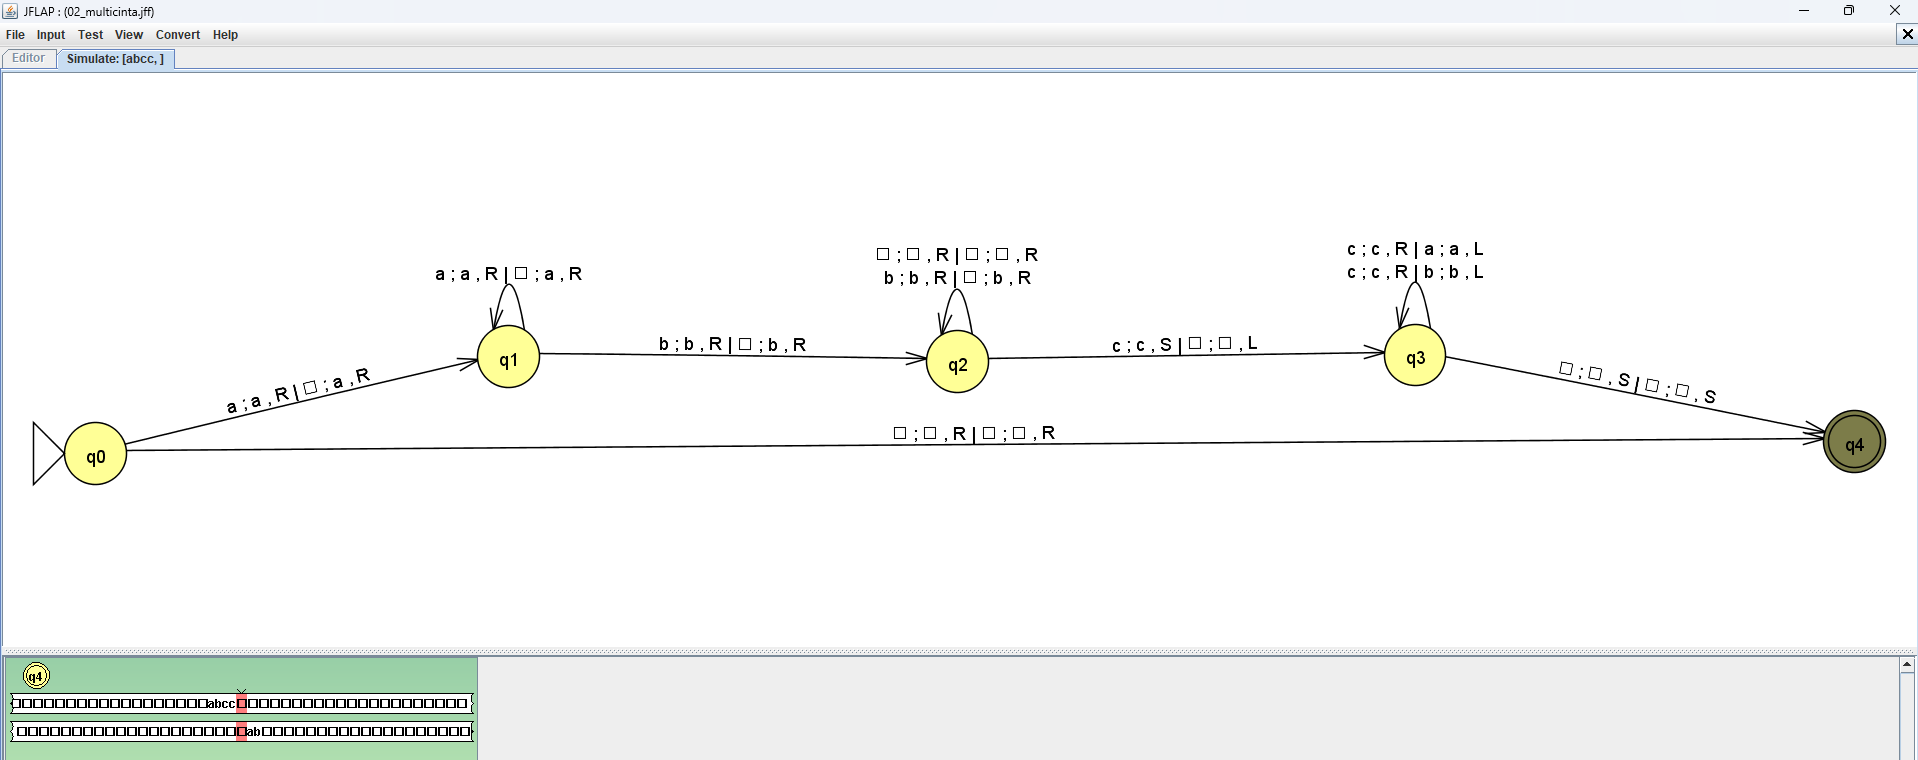
\includegraphics[scale=0.3]{img/MT_02_multiple_ribbon_simulation_2.png}
          \caption{Simulación de la máquina de Turing que acepta el lenguaje $L = \{a^nb^mc^{n+m} \mid n \geq 0, m \geq 0\}$ de dos cintas.}
        \end{figure}
\end{itemize}

\newpage

% Ejercicio 3
\section{Diseñar y simular en JFLAP máquinas de Turing que acepten el lenguaje $L = \{a^nb^mc^{n*m} \mid n \geq 1, m \geq 1\}$}
% \subsection{Diseño de una cinta}
% \begin{itemize}
%   \item \textbf{Descripción y diseño:} Esta máquina de Turing tiene una cinta, lo que hace es ir marcando por cada $a$ una $c$ y por cada $b$ una $c$. Luego, regresa al inicio de la cadena y repite el proceso hasta que no haya más $a$'s y $b$'s. Cuando termina de procesar la cadena, la máquina verifica que no haya caracteres restantes sin marcar. El diseño de la máquina de Turing es el siguiente:

%         \begin{figure}[H]
%           \centering
%           \includegraphics[scale=0.33]{img/MT_03_one_ribbon.png}
%           \caption{Máquina de Turing que acepta el lenguaje $L = \{a^nb^mc^{n*m} \mid n \geq 1, m \geq 1\}$ de una cinta.}
%           \label{fig:maquina de turing que acepta el lenguaje L = {a^nb^mc^{n*m} | n >= 1, m >= 1}}
%         \end{figure}

%   \newpage

%   \item \textbf{Simulación:} La simulación de la máquina de Turing con algunas cadenas:
%         \begin{figure}[H]
%           \centering
%           \includegraphics[scale=0.33]{img/MT_03_one_ribbon_simulation.png}
%           \caption{Simulación de la máquina de Turing que acepta el lenguaje $L = \{a^nb^mc^{n*m} \mid n \geq 1, m \geq 1\}$ de una cinta.}
%           \label{fig:simulacion de la maquina de turing que acepta el lenguaje L = {a^nb^mc^{n*m} | n >= 1, m >= 1}}
%         \end{figure}
% \end{itemize}

% \newpage

% \subsection{Diseño de multiples cintas}
% \begin{itemize}
%   \item \textbf{Descripción y diseño:} Esta máquina de Turing tiene dos cintas, la primera se encarga de procesar la cadena y la segunda en hacer una copia de tantos $a$'s que hay y luego así contar si hay el mismo número de $b$'s y $c$'s. El diseño de la máquina de Turing es el siguiente:

%         \begin{figure}[H]
%           \centering
%           \includegraphics[scale=0.3]{img/MT_03_multiple_ribbon.png}
%           \caption{Máquina de Turing que acepta el lenguaje $L = \{a^nb^mc^{n*m} \mid n \geq 1, m \geq 1\}$ de dos cintas.}
%           \label{fig:maquina de turing que acepta el lenguaje L = {a^nb^mc^{n*m} | n >= 1, m >= 1}}
%         \end{figure}

%   \newpage

%   \item \textbf{Simulación:} La simulación de la máquina de Turing con algunas cadenas:
%         \begin{figure}[H]
%           \centering
%           \includegraphics[scale=0.3]{img/MT_03_multiple_ribbon_simulation.png}
%           \caption{Simulación de la máquina de Turing que acepta el lenguaje $L = \{a^nb^mc^{n*m} \mid n \geq 1, m \geq 1\}$ de dos cintas.}
%           \label{fig:simulacion de la maquina de turing que acepta el lenguaje L = {a^nb^mc^{n*m} | n >= 1, m >= 1}}
%         \end{figure}
% \end{itemize}

\newpage

% Ejercicio 4
\section{Diseñar y simular en JFLAP máquinas de Turing que acepten el lenguaje \(L = \{w \mid w = w^{-1}\}\) sobre el alfabeto \(\Sigma = \{0, 1\}\)}
\subsection{Diseño de una cinta}

\end{document}